\section{Problem Definition}

We formally define the cross-modal truth discovery problem in this section.
Consider a scenario where a group of users report a specific type of spatio-temporal events (e.g., traffic jam, accident). A user $u$
makes an observation $o$ at time $t$. Each observation $o=(u,l,t,d,c)$ contains the user ID $u$, the location $l$ of the event (e.g., by GPS), the time $t$ of the observation, and the description of the event. The description is a list of  text, keywords or hashtags and  a set of modal features characterizing the content $c$. 

For example, the image  in Fig. 1 posted on Flickr is the content of one observation made by user $Phic$ on Oct. 30, 2013,  around 2 pm, related to traffic at the intersection of Markhiya and Al Bidda roads in Doha, Qatar. This observation is  encoded as: \\
$('Phic', gpslong,gpslat, dateformat,text, imageBLOB )$  to complete

%-----------------------------------
\begin{figure}[t]
 \centerline{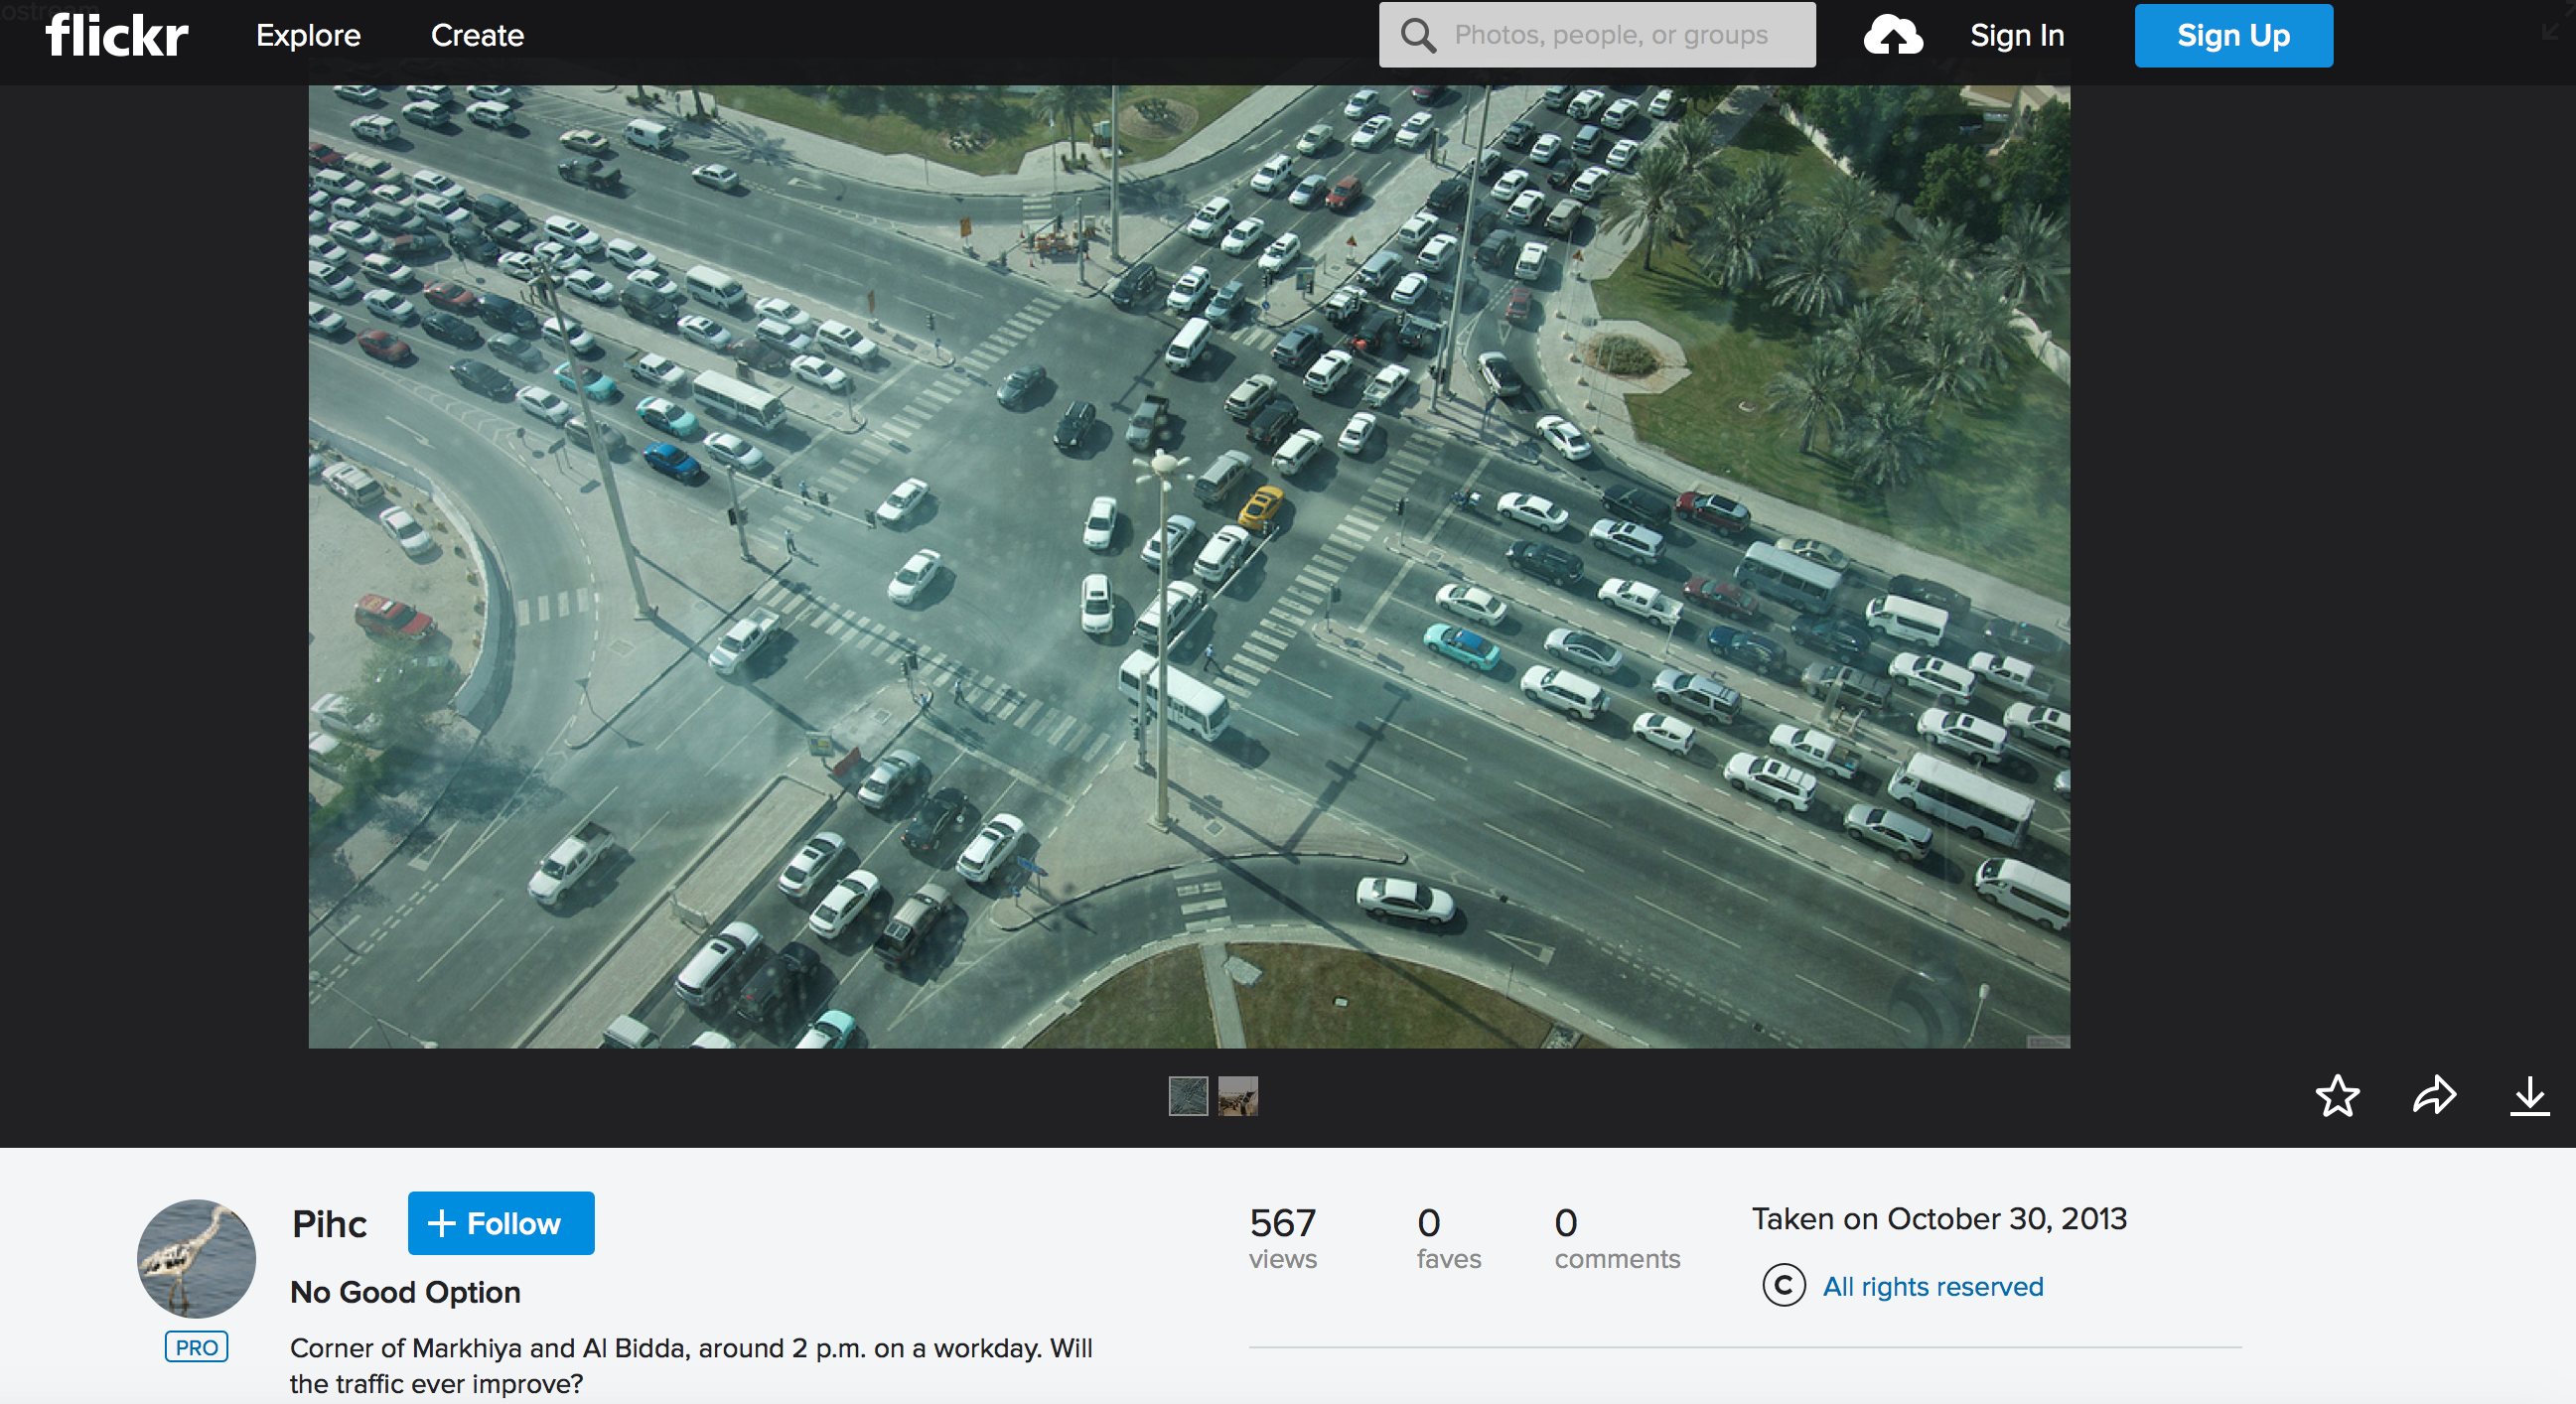
\includegraphics[scale=.45,width=.45\textwidth]{fig-example.png}}
\caption{ Example of observation}
\label{fig1}
\end{figure}
%-----------------------------------

We consider the set of observations collected within a certain time window $\mathcal{T}$ and a spatial
region of interest $\mathcal{S}$ such as:
$$ \mathcal{O}=\{ o \mid o.t \in\mathcal{T}, o.l \in\mathcal{S} \}.$$

  Given $ \mathcal{O} $, the problem we address is first to group together the observations that are most likely referring to the same real-world event (blocking/linking). Second, among the candidate observations linked to a given event, our goal is to infer the most accurate time, location, and description of the event.

